\section{Introduction}
%Wireless signals, such as WiFi and the radio frequency (\RF), have emerged as a cheap yet powerful medium for information sensing. By
%measuring how the wireless signal is affected by surrounding objects and human activities, tasks like gait identification~\cite{}, gesture
%recognition~\cite{}, activity recognition~\cite{}, and vital sign monitoring~\cite{} can be possible.
%
%
%The desire for employing wireless signals for sensing could date back to the 19th century  for the discovery of X-rays for object
%recognition~\cite{} and the development of military radar and sonar systems for tracking large metallic objects in open
%spaces~\cite{Charles Samuel Franklin 's development of first practcial radar}. These sensing systems, however, have to rely on expensive specialize hardware and be operated by professionals, which thus put they out of the reach of ordinary people.
%
%
%Recently, it has been shown that wireless sensing built upon consumer-grade devices such as smartphones and wireless routers can be used to
%precisely track human activities in an indoor environment. Such technology has the advantages of being low-cost as it requires as few as
%two wireless routers to operate, not requiring instrumenting the user, being less privacy intrusive compared to other infrastructure-based
%solutions like video-based solutions~\cite{}, and is safer to use on a regular basis compared to other alternatives like X-rays~\cite{}. It
%offers an inexpensive way for bringing activity sensing into everyday life -- which not only makes ever sensing a tantalizing reality but
%could also open up new possibilities for innovative applications.
%
%
%As we will show in this article, while there are still many challenges ahead, consumer-grade wireless sensing has moved from a research
%niche to a mainstream activity. This is, in fact, a dynamic field looking at subjects as diverse as smart-home personalization~\cite{} and
%fall monitoring~\cite{} to emotion detection~\cite{}. In this article we aim to demystify this promising technique, outline the challenges
%it is facing, and show that this is a trustworthy and exciting research direction.
%
%
%
%
%The remainder of this article is structured as follows. We first give an intuitive view for the wireless sensing working mechanism  in
%Section~\ref{sec:mechanism}. \FIXME{We then describe xx, bla bla...}. We discuss the challenges and limitations for wireless sensings, as
%well as open research directions in Section xx before we summarise and conclude in Section \FIXME{xx}.



%Wireless technologies have achieved a great success in data communication, changing our lives in every aspect. 
Sensing technologies play a key role in the internet of things~(IoT), changing our lives in every aspect. Recent years have witnessed a surge in artificial intelligence. Great success have been made both in respects of accuracy and robustness. In particular, wearable sensing systems hold robust performance, however they are inconvenient sometimes since the devices that users have to wear~\cite{Pinpoint}. In contrast, vision-based sensing using cameras has revolutionized the field of human-computer interaction via enabling 3D tracking without instrumenting the object~\cite{Cruz2015Quantification}. Yet these systems have the fundamental limitations of requiring obstacle-free and breaching human privacy potentially.

In the last few years, pervasive wireless signals such as \WiFi, \RFID and sound, have emerged as a powerful medium to sense the human and also the surrounding environment. Wireless sensing has enabled a large variety of exciting new applications including indoor localization~\cite{Arraytrack,
Tagoram}, activity/gesture recognition~\cite{Wang2015Understanding, wang2016human}, fall detection~\cite{wang2017wifall}, respiration monitoring~\cite{Smart-homes}, emotion sensing~\cite{Zhao2017Emotion},  material identification~\cite{Tagscan, LiquID}, room layout mapping~\cite{Lu2018}, imaging~\cite{zhao2018rf}, etc.


The history of using wireless signals for sensing dates back to the 19th century when people utilize X-rays for imaging~\cite{Suzuki1996} and developed radar and sonar systems for tracking large metallic objects in open
spaces~\cite{Au1988Sonar}. Though powerful, these sensing systems, however, employ expensive specialized hardware and need to be operated by professionals, putting them out of the reach of ordinary people.
Recently, wireless signals generated by cheap commercial off-the-shelf (COTS) hardware such as smartphone, \WiFi access point and \RFID reader are demonstrated to be able to
sense the human activity, image the target, monitor the subtle respiration movement and identify the material type of object as shown in Fig.~\ref{fig:scenarios}.  % track objects and human activities in an indoor environment, as shown in Fig.~\ref{fig:scenarios}. Such technology has the advantages of being low-cost as it
%requires as few as two wireless routers to operate, not requiring instrumenting the user,
%Contactless wireless sensing exhibits clear advantage of less intrusive compared to wearable-based sensing and does not compromise people privacy compared to video-based solutions~\cite{Cruz2015Quantification}. %Compared to the expensive and is safer to use on a regular basis compared to other alternatives like X-rays~\cite{De2013B}.
We envision wireless sensing has a tremendous potential to be widely adopted in many of our everyday applications in the Era of IoT. % capabilities into everyday life, making
%ever sensing a tantalizing reality.

As we will show in this article, while there still remain unaddressed challenges, wireless sensing has achieved promising progresses and we believe this is an exciting and at the same time rewarding direction for researchers to explore.

%with CTOS hardware has moved from a research niche to a mainstream activity. This is, in fact, a dynamic field looking at subjects as diverse as smart-home personalization~\cite{vasisht2016decimeter} and
%fall monitoring~\cite{wang2017wifall} to emotion detection~\cite{Zhao2017Emotion} and vital sign monitoring~\cite{Smart-homes}. In this article we aim to demystify this promising
%technique, outline the challenges it is facing, and show that this is a trustworthy and exciting research direction.


\begin{figure} [t!]
\centering
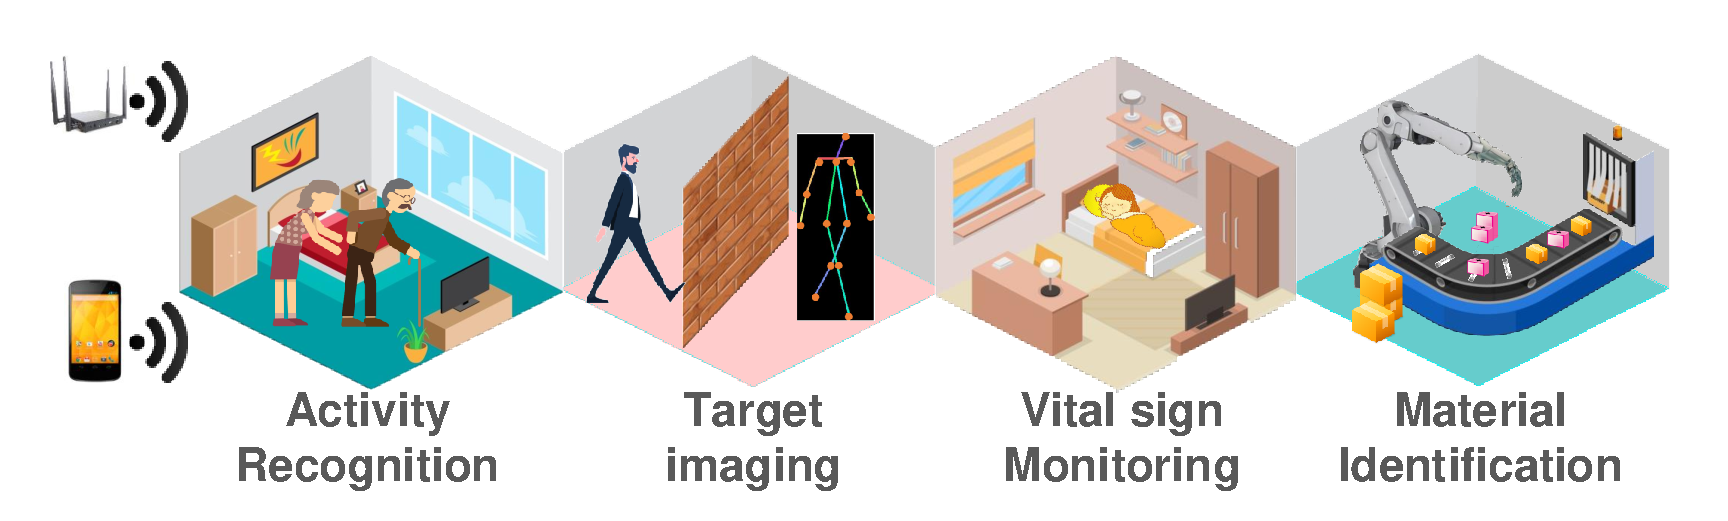
\includegraphics[width=0.5\textwidth]{figures/scenarios.pdf}
\caption{Examples of wireless sensing.}
\label{fig:scenarios}
\end{figure}


